
\begin{frame}
\titlepage % Print the title page as the first slide
\end{frame}

% \begin{frame}
% \frametitle{Agenda} % Table of contents slide, comment this block out to remove it
% \tableofcontents % Throughout your presentation, if you choose to use \section{} and \subsection{} commands, these will automatically be printed on this slide as an overview of your presentation
% \end{frame}

%----------------------------------------------------------------------------------------
%   PRESENTATION SLIDES
%----------------------------------------------------------------------------------------

%------------------------------------------------
\begin{frame}
% \section{Objetivo do Projeto} % Sections can be created in order to organize your presentation into discrete blocks, all sections and subsections are automatically printed in the table of contents as an overview of the talk
%------------------------------------------------
\frametitle{Objetivo do Projeto}

\begin{itemize}
	\item Desenvolver sistema de roteamento orientado a contexto capaz de:
	\begin{itemize}
		\item Perceber, inferir e aprender com as informações obtidas por sensores de um certo ambiente/contexto.
		\item Selecionar, com isso, a melhor rota para envio de dados.
		\item Demonstrar conceitos de sensibilidade ao contexto para criação de dispositivos inteligentes.
	\end{itemize}
\end{itemize}
\end{frame}

% \subsection{Subsection Example} % A subsection can be created just before a set of slides with a common theme to further break down your presentation into chunks

\begin{frame}
\frametitle{Arquitetura}
\begin{itemize}
	\item Linguagens utilizadas
	\item Python e Shell (Bash)
	\item Protocolo de camada 2
	\item ÍEEE 802.11 g/n
	\item Protocolo de roteamento
	\item OSPF no Quagga
	\item Hardware:
	\item Raspberry Pi 3 (Raspbian/Debian Linux)
\end{itemize}

\end{frame}

%------------------------------------------------

\begin{frame}
	\frametitle{Camadas do sistema}

	\begin{figure}[h]
		\centering
		% 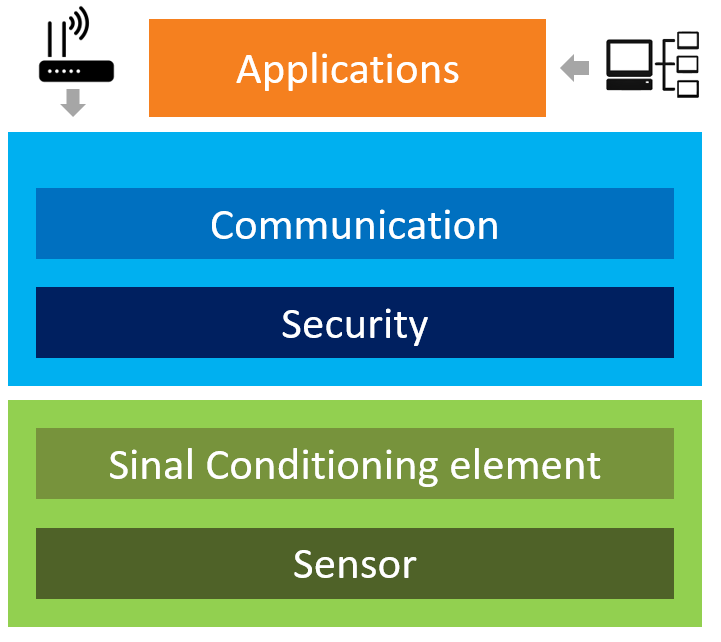
\includegraphics[width=0.3\textwidth]{"../Relatorio/Artigo IoT-G4/figs/system-layer.png"}
		% \caption{System Layers}
		\label{System-Layers}
 	\end{figure}

\end{frame}

%------------------------------------------------

\begin{frame}
	\frametitle{Topologia}
\end{frame}

%------------------------------------------------

\begin{frame}
	\frametitle{Sensores}

\begin{description}
	\item [DHT11] Umidade e Temperatura
	\begin{itemize}
		\item Leituras de temperaturas entre 0 a 50$^o$ Celsius e umidade entre 20 a 90\%.
	\end{itemize}
	\item [LDR] Luminosidade
	\begin{itemize}
		\item O LDR(\textit{Light Dependent Resistor}) possui uma característica que faz com que sua resistência varie conforme a luminosidade incendida  sobre ele.
	\end{itemize}
\end{description}

\end{frame}

%------------------------------------------------


\begin{frame}
	\frametitle{Sensores - Circuito}

\begin{figure}[!tb]
\begin{center}\begin{circuitikz}[scale=0.9]
  \draw (0,0) -- (0,2) to [R=10<\kilo\ohm>,*-*] (2,2);
  \draw (0,2) -- (0,3) to [R=10<\kilo\ohm>,*-*] (2,3);
  \draw (0,3) to[short,*-o] (0,5) node[above]{$V_{CC}=3.3V$}; % Power supply
  \draw (0,4) to[short,*-] (1.9,4) -- (1.9,4.5);
  \draw (0,0) to [phR=LDR,*-*](2,0) to [eC,l=10<\micro\farad>,*-*](4,0) -- (4,4) -- (2.2,4) -- (2.2,4.5);
  \draw (4,3.5) to[short,*-] (4.5,3.5) node[ground]{};
  \draw (2,2) -- (2,4.5);
  \draw (2.1,4) -- (2.1,4.5);
  \draw (1.4,5.7) rectangle (2.7,4.5)
    node at(2.05,5.1){DHT11};
   %gpio pins
  \draw (2,0) to[short,*-o] (2,-1) node[right]{Pin11};
  \draw (2,2) to[short,*-o] (2.5,2) node[right]{Pin7};

 \end{circuitikz} \end{center}
% \caption{Sensor circuit}
\label{sensor-circuit}
\end{figure}

\end{frame}

%------------------------------------------------

\begin{frame}
	\frametitle{Funcionamento}
\end{frame}

%------------------------------------------------

\begin{frame}
	\frametitle{Dados Coletados - Sensores}
\end{frame}

%------------------------------------------------

\begin{frame}
	\frametitle{Resultados Experimentais}
\end{frame}

%------------------------------------------------

\begin{frame}
	\frametitle{Resultados Experimentais}
\end{frame}

%------------------------------------------------

\begin{frame}
	\frametitle{Resultados Experimentais}
\end{frame}

%------------------------------------------------

